\chapter{\poy Quick Start}

\section{What is \poy}

\poy is a flexible, multi-platform program for phylogenetic analysis of molecular and other data under various optimality criteria. An essential feature of \poy is that it implements the concept of dynamic homology allowing optimization of unaligned sequences. \poy offers great flexibility for designing heuristic search strategies and implements an array of algorithms including swapping, tree fusing, tree drifting, and ratcheting. As output, \poy generates a comprehensive character diagnosis, graphical representations of cladograms and their user-specified consensus, as well as support values, and implied alignments. \poy provides a unified approach to co-optimizing different types of data, such as morphological and molecular sequence data. In addition, \poy can analyze entire chromosomes and genomes and take into account large-scale genomic events (translocations, inversions, and duplications).

Currently \poy is beta software, and therefore it has some known glitches. Most
of them will be worked out in the following months, and updated versions will be
available on the program's webpage as we produce them. Our current schedule of
work expect to have a final official version of the parsimony components of the
program and a release of the beta components of the maximum
likelihood components in mid may of 2007. For the list of known issues see the
Section~\ref{sec:known_issues}.

\section{The structure of \poy documentation}
The first chapter, \emph{\poy Quick Start}, will get you started using \poy. The first few sections are intended to provide detailed instructions on how to obtain and install \poy, introduce the user to the program's two working environments, the \emph{Graphical User Interface} and \emph{POY Interactive Console}. These sections also show how to initiate a \poy session and point to the various resources to obtain further assistance. Subsequent sections (starting with \emph{1.13 Using \poy}) build on that knowledge and give step-by-step examples on how to conduct a basic analysis and visualize the results. The \emph{\poy Quick Start} is not a tutorial on \poy; using \poy assumes a knowledge of \poy commands and their valid syntax that are detailed in the second chapter, \emph{\poy Commands}. More advanced operations are described in the third chapter, \emph{\poy Tutorials}. In addition to the general index, this document contains a \emph{\texttt{POY3.0} Command Line Index}, intended to provide a link between the commands used in \texttt{POY3} and the commands used in \poy. 

The Quick Start is created primarily for a typical user with limited experience using command-line applications and assumes little or no knowledge of Unix. Consequently, certain operations suggested here could be performed more efficiently by an experienced user, but in attempt to make the software as accessible as possible, we provide simple and intuitive step-by-step (platform-specific where necessary) instructions. 

\section{Requirements: software and hardware}

\subsection{Software}
\poy is a platform-independent, open-source program that is compiled for Mac OSX, Microsoft Windows, and Linux systems. \poy \emph{binaries}\index{general}{binaries} (compiled application file) is the only piece of software necessary to run \poy. Other utility programs (that are typically installed with major operation systems), can facilitate preparation of \poy scripts (\poy command batch files) and formatting datafiles.

\begin{flushleft}
	\begin{minipage}[c]{0.074\textwidth}
	   	
\includegraphics[width=\textwidth]{figures/figLogoWindows.jpg}
	\end{minipage}%
	\quad
	\begin{minipage}[t]{0.88\textwidth}
		   	\subsubsection{Windows}
	\end{minipage}
		\begin{description}
			\item[Notepad] is a basic text editor that can be used to create \poy
			scripts and format datafiles. By default, it is located in the \emph{Accessories}
			folder under \emph{All Programs} of the \emph{Start} menu.
			\item[Command Prompt] provides a working environment for
			\poy and is used to initiate a \poy session.
		It can be accessed from the same \emph{Accessories} folder as Notepad.
		\end{description}

	\begin{minipage}[c]{0.074\textwidth}
   		
\includegraphics[width=\textwidth]{figures/figLogoMac.jpg}
	\end{minipage}%
	\quad
	\begin{minipage}[t]{0.88\textwidth}
	   	\subsubsection{Mac OSX}
	\end{minipage}
			\begin{description}
				\item[Terminal]  is an interface for UNIX operating systems and it
				provides a working environment for \poy; it is used to initiate a
				\poy session. Terminal is located in the \emph{Utilities} folder within
				the \emph{Applications} folder. (The program X11, that is
				also provided with OS X, can be used as an alternative to Terminal.)
				\item[TextEdit] is a basic text editor that can be used to create \poy
				scripts and format datafiles. By default, it is located in the
				\emph{Applications} folder. More flexible text editors, such as
				shareware applications like BBEdit or TextWrangler, are good alternatives.
			\end{description}		

	\begin{minipage}[c]{0.074\textwidth}
   		
\includegraphics[width=\textwidth]{figures/figLogoLinux.jpg}
	\end{minipage}
	\quad
	\begin{minipage}[t]{0.88\textwidth}
	   	\subsubsection{Linux} 
	\end{minipage}

    A simple text editor, such as \href{http://www.nano-editor.org/}{\emph{nano}}, is sufficient, though more powerful
    editors (such as \href{http://www.vim.org}{\emph{vim}} or
    \href{http://www.gnu.org/software/emacs/}{\emph{emacs}}) can make your life much
    easier writting scripts for \poy.

\end{flushleft}

\subsection{Hardware}
\poy runs on a variety of computers computers from laptops and desktops to Beowulf clusters 
of various sizes to symmetric multiprocessing hardware. There are no
particular requirements for disk space. Processor speed and memory (and
communications bandwidth and latency in parallel environments) are important.
Depending on the size and complexity of the data, and the computational
complexity of requested operations, a \poy session can consume large amounts of memory.
However, the flexible structure of \poy allows for partitioning of individual
tasks to prevent overwhelming the hardware. Strict guidelines cannot be
provided because the performance depends on the specifics of a given
dataset; however, one can estimate the memory requirements by running a test command
or script under less demanding settings.

\section{Obtaining and installing \poy}

Compressed files of \poy binaries, source code, and documentation in PDF format are available 
for various Linux distributions, Microsoft Windows XP, and Mac OSX Tiger at the American Museum 
of Natural History Computational Sciences \poy website:
\begin{center}
\url{http://research.amnh.org/scicomp/projects/poy.php}
\end{center}
The following detailed step-by-step instruction will guide you through downloading,  decompressing, and installing \poy binaries for various platforms.

\begin{flushleft}
	\begin{minipage}[c]{0.074\textwidth}
	   	
\includegraphics[width=\textwidth]{figures/figLogoWindows.jpg}
	\end{minipage}
	\quad
	\begin{minipage}[t]{0.88\textwidth}
		   	\subsubsection{Windows}
	\end{minipage}
		\begin{itemize}
			\item
                Download the
                \href{http://research.amnh.org/scicomp/projects/poy.php}{Windows compressed binary} file to the desktop.

			\item 
                Open the zipped file and run the windows installer
                POY\_installer.msi. The installer will create shortcuts in the
                \emph{Programs} menu.
		\end{itemize}

	\begin{minipage}[c]{0.074\textwidth}
   		
\includegraphics[width=\textwidth]{figures/figLogoMac.jpg}
	\end{minipage}
	\quad
	\begin{minipage}[t]{0.88\textwidth}
	   	\subsubsection{Mac OSX}
	\end{minipage}
	            \begin{itemize}
			\item Download the
            \href{http://research.amnh.org/scicomp/projects/poy.php}{disk
            image} file to the desktop and open it. A disk named \emph{poy4} will be
            mounted.
            		\item Drag the \poy application from the
            disk \emph{poy4} and drop it into the \emph{Applications}
            folder on the hard drive.
		\end{itemize}

	\begin{minipage}[c]{0.074\textwidth}
   		
\includegraphics[width=\textwidth]{figures/figLogoLinux.jpg}
	\end{minipage}
	\quad
	\begin{minipage}[t]{0.88\textwidth}
	   	\subsubsection{Linux}
	\end{minipage}
		\begin{itemize}
			\item  Download the 
    \href{http://research.amnh.org/scicomp/projects/poy.php}{gzipped} file.
    			\item Untar and ungzip the \emph{poy4.tar.gz} file.
			\item Run the command \texttt{tar -Pxvzf poy4.tar.gz} as a
    super user in the newly created \emph{poy4} directory.
    The GUI will be installed in \texttt{/opt/poy4/Contents/POY} directory
    and terminal binaries in \texttt{/opt/poy4/Resources/ncurses\_poy} directory.
		\end{itemize} 

\end{flushleft}

\subsubsection{Compiling from the Source}

In order to compile \poy the following tools are required:

\begin{enumerate}
    \item \href{http://www.gnu.org/software/make/}{The GNU Make tool.}
    \item \href{http://www.ocaml.org}{OCaml version 3.10.0. or later.}
    \item \href{http://gcc.gnu.org/}{A C compiler, for example The GNU Compiler Collection}.
    \item \href{http://www.gnu.org/software/ncurses/}{The ncurses library} if
        you want the nice interactive console, thought this one is
        \emph{not obligatory}.
    \item \href{http://tiswww.case.edu/php/chet/readline/rltop.html}{The
        readline library} if you want
        to compile POY without interactive console. This is the typical
        selection when compiling POY for parallel environments under MPI.
\end{enumerate}

Download, ungzip, and untar the
\href{http://research.amnh.org/scicomp/projects/poy.php}{\poy source code};
In order to compile under default setting just do:
\begin{verbatim}
./configure
make
make install
\end{verbatim}
All the configuration options can be found in {\tt ./configure --help}.

\poy can also be run in parallel environments using the
\href{http://www-unix.mcs.anl.gov/mpi/}{Message Passing Interface}. There are
multiple implementations, and if you have a parallel environment, most likely
your system administrator has already installed one. Ask him for the proper
paths to set in your config file.

\section{The Graphical User Interface}

\poy provides two working environments: the \emph{Graphical User Interface} and the \emph{Interactive Console}.  The \emph{Graphical User Interface} has a user-friendly appearance as any other native stand-alone application where different functions are accessible through menus and windows. Thus, the entire analysis can be carried out clicking on appropriate selections and, where necessary, typing specifications in designated fields. Although intuitive and accessible, the the \emph{Graphical User Interface} does not provide all the available options and is not as flexible for designing a search strategy as \emph{Interactive Console}. The interactive console, however, requires a detailed knowledge of \poy commands, their arguments, and the conventions of \poy scripting. All these features are described in detail in the \emph{POY Commands} chapter.

Even though the Mac OSX version of the \emph{Graphical User Interface} is used for screen shots throughout this chapter, its Linux and Windows versions contain the same items and functionality, differing only by the generic window format specific to each platform.

When \poy is first open, two items appear on the screen: the menu bar across the top and the \emph{POY Launcher} window (Figure~\ref{fig:menu_launcher_window}). Note that in Linux the menu bar is within the launcher window.
\begin{figure}[htpb]
    \begin{center}
        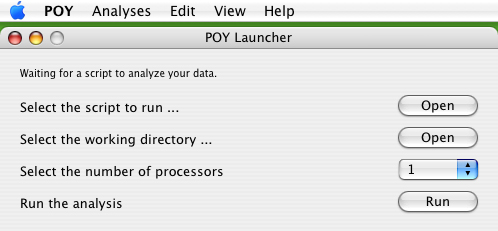
\includegraphics[width=0.5\textwidth]{figures/menu_launcher_window.jpg}
    \end{center}
    \caption{The \poy menu bar and the \emph{POY Launcher} window. These items appear when \poy is opened.}
    \label{fig:menu_launcher_window}
\end{figure}

\subsection{POY menu bar}
The menu bar contains the following drop-down menus:
\begin{description}
\item[POY] This menu is present only in Mac OSX and contains generic items as other Mac OSX applications. It includes \emph{Quit POY} tap that closes the program. This menu also allows to display the \emph{About POY} window (Figure~\ref{fig:about_window}) which lists the current version of \poy, a copywright statement, and the address of \poy website.
\item[Analysis] This menu contains options for different types of tree searches, calculation of support values, tree diagnosis, and their respective outputs. Other items in this menu open the \emph{POY launcher} and the \emph{Interactive Console}.
\item[Edit] This menu contains standard tools for deleting, copying, cutting, pasting, undoing, and selecting.
\item[View] Selecting items in this menu opens \emph{Results} and \emph{Status} windows that display, respectively, the results and the current state of the analysis.
\item[Help] This menu provides a link to the \poy \emph{QuickStart and Program Documentation} in PDF format.
\end{description}

\subsubsection{About POY}

The about window contains the program version number and contact information for
the program. It can be found in the \poy menu of Mac OS X, or the \emph{View} menu of
Windows and Linux.
\begin{figure}[htpb]
    \begin{center}
        
\includegraphics[width=0.35\textwidth]{figures/About_Window.jpg}
    \end{center}
    \caption{The \emph{About POY} window.}
    \label{fig:about_window}
\end{figure}

\subsection{POY Launcher} 
\emph{POY Launcher} is the only window that automatically opens upon starting
\poy. It allows the user to import a previously created script,
designate a working directory, specify the number of processors,
and start the analysis.

\begin{description}
	\item[Select the script to run...]
     Allows the user to specify the location of a \poy script.
	\item[Select the working directory...]
    By default the working directory is set to be the same as the
    directory containing the selected \poy script but the default
    can be modified by the user. The working directory is the
    directory that contains the data files and where the results
    are reported.
	\item[Select the number of processors]
    The selection of the number of processors is disabled for LINUX
    and WINDOWS platforms. Once specified, the selection is applied
    to all subsequent analyses in the current \poy session.
	\item[Run the analysis]
    Clicking the \emph{Run} button starts the execution of the selected
    script. Once the script is executed, the \emph{Run} button
    becomes the \emph{Cancel} button that can be used to interrupt
    a \poy session.
\end{description}

If the script is executed without the properly selected script and
working directory (of their names contain errors), \poy issues an
error message in the upper part of the \emph{POY Launcher} window,
such as \texttt{POY finished with an error}.

\subsection{The \emph{Analysis} menu}
The \emph{Analysis} menu is the main toolbox of \poy. Its selections are subdivided into four functional categories that deal with tree searching, support calculation, tree diagnosis, and data import (including the initialization the \emph{Interactive Console}). Each of the menu items is described below in order as it
appears on the menu. Most options are the same for different kinds of analysis. Therefore, all the options are described in detail only for the \emph{Simple Search} analysis. The descriptions of other analyses is made with reference to the the \emph{Simple Search} and focus on options unique to each kind of analysis.

\subsubsection{\emph{Tree searching options}}

\subsubsection{Simple Search}
The \emph{Simple Search} window (Figure~\ref{fig:simple_search_window})
provides the most common and basic options for a standard tree search
in \poy that must either (in some cases or) selected by clicking appropriate buttons or typed in. Note that \emph{all} the empty fields must be filled out. The window is subdivided in four sections: 

\begin{figure}
\centering
\begin{minipage}[c]{0.48\textwidth}
   		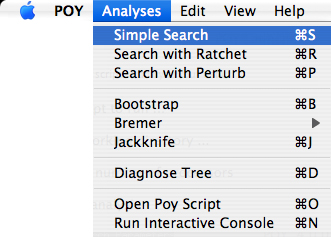
\includegraphics[width=\textwidth]{figures/SimpleSearch_Menu.jpg}
\end{minipage}
\quad
\begin{minipage}[c]{0.48\textwidth}
	   	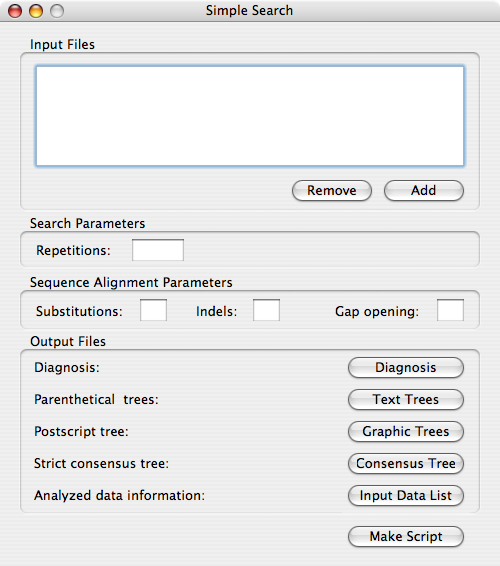
\includegraphics[width=\textwidth]{figures/SimpleSearch_Window.jpg}
   	\end{minipage}
	
\caption{The \emph{Simple Search} window. Selecting \emph{Simple Search} from the \emph{Analysis} menu (left) and viewing the \emph{Simple Search} window options (right).}
\label{fig:simple_search_window}
\end{figure}

\begin{description}
    \item[Input Files]
        Contains the list of files that are to be read by \poy. These include
        character files, and tree files. 
    \item[Search Parameters]
        Sets the number of randomized trees (independent random addition replicates)
        to be generated.
    \item[Sequence Alignment Parameters]
        Specifies the substitution, indel, and gap opening costs. Enter \texttt{0} if no
        gap opening cost is desired.
    \item[Output Files]
        Designates the names and locations of files containing different kinds of results
        (implied by their respective titles) of the analysis.
\end{description}

Once all the parameters are selected, click the \emph{Make Script} button and another
window--the \emph{Script Editor}--containing the generated script appears on screen. The
script can be edited by typing in the commands directly in the \emph{Script Editor} window,
 saved (by clicking the \emph{Save As} button), or replaced with another script (using 
 the \emph{Open} button. To start the analysis click the \emph{Run} button in the 
 \emph{Script Editor} window. When the \emph{Run} button is pressed, \poy will issue a
 request to  to save the script to be executed. Thus, not only does \poy execute the script but
 it also created the record of what kind of analysis (including all user-defined specifications) was performed.
 
 \begin{figure}[htpb]
    \begin{center}
        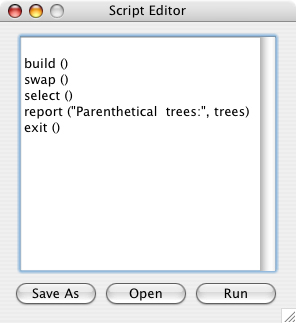
\includegraphics[width=0.5\textwidth]{figures/ScriptEditor_Window.jpg}
    \end{center}
    \caption{Viewing the \emph{Script Editor} window. The script was generated from the \emph{Simple Search} window by clicking the \emph{Make Script} button. Because no fields were filled, the script does not contain the input files and shows the commands under default settings that would be executed under a simple search strategy.}
    \label{fig:ScriptEditor_Window}
\end{figure}

\subsubsection{Search with Ratchet}

\emph{Search with Ratchet} (Figure~\ref{fig:search_with_ratchet_window}) provides means to escape the local optimum using the parsimony ratchet. In addition to the same four parameter groups described for the \emph{Simple Search} window, the \emph{Search Parameters} section provides the following ratchet parameters fields:

\begin{figure}
\centering
\begin{minipage}[c]{0.48\textwidth}
   		\includegraphics[width=\textwidth]{figures/SearchWithRatchet_Menu.jpg}
\end{minipage}
\quad
\begin{minipage}[c]{0.48\textwidth}
	   	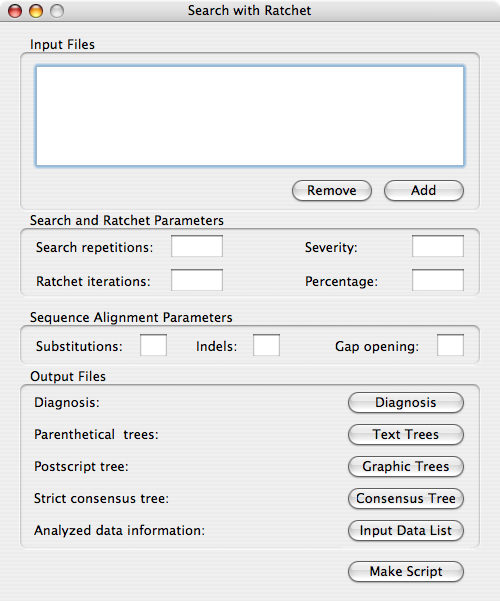
\includegraphics[width=\textwidth]{figures/SearchWithRatchet_Window.jpg}
   	\end{minipage}
	
\caption{The \emph{Search with Ratchet} window. Selecting \emph{Search with Ratchet} from the \emph{Analysis} menu (left) and viewing the \emph{Search with Ratchet} window options (right).}
\label{fig:search_with_ratchet_window}
\end{figure}

\begin{description}
    \item[Ratchet iterations] The number of iterations for the parsimony
        ratchet.
    \item[Severity] The severity parameter of the parsimony ratchet (the weight
        change factor for the selected characters).
    \item[Percentage] The percentage of characters to be affected by the
        parsimony ratchet.
\end{description}

\subsubsection{Search with Perturb}

\emph{Search with Perturb} provides a different way to escape the local optima by changing
the transformation cost matrix of the molecular characters
(Figure~\ref{fig:search_with_perturb_window}). In addition to the
same four parameter groups described for the Simple Search window, the Search
with Perturb window provides three extra fields with the parameters for the
transformation cost matrix perturbation as follows:

\begin{figure}
\centering
\begin{minipage}[c]{0.48\textwidth}
   		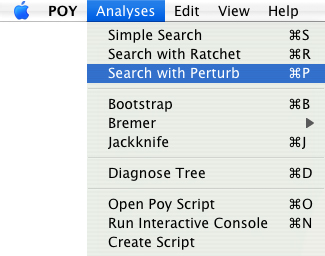
\includegraphics[width=\textwidth]{figures/SearchWithPerturb_Menu.jpg}
\end{minipage}
\quad
\begin{minipage}[c]{0.48\textwidth}
	   	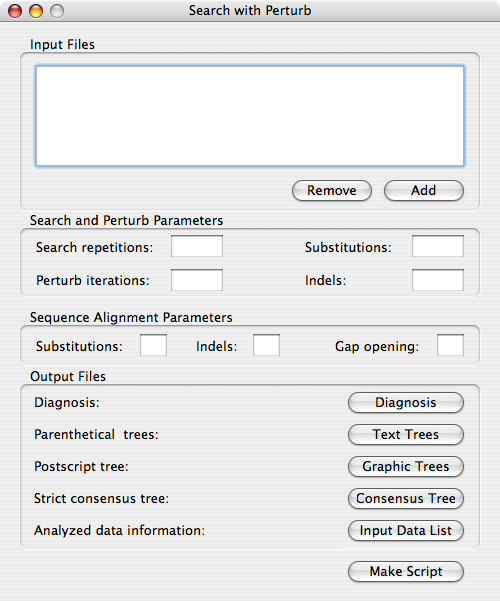
\includegraphics[width=\textwidth]{figures/SearchWithPerturb_Window.jpg}
   	\end{minipage} 
\caption{The \emph{Search with Perturb} window. Selecting \emph{Search with Perturb} from the \emph{Analysis} menu (left) and viewing the \emph{Search with Perturb} window options (right).}
\label{fig:search_with_perturb_window}
\end{figure}

\begin{description}
    \item[Perturb iterations] Sets the number of perturb iterations to be performed.
    \item[Substitutions] Specifies the cost of the perturbed substitutions.
    \item[Indels] Specifies the cost of the perturbed indels.
\end{description}

\subsubsection{\emph{Support calculation options}}

None of the support calculation windows include functions for tree building and searching. Therefore, one of the input files must contain trees for which support values are going to be calculated.

\subsubsection{Bootstrap}

The \emph{Bootstrap} window specifies parameters
for estimating the Bootstrap support values. The window consists
of essentially same four sections as the \emph{Simple Search} window
except for \emph{Pseudoreplicates}, a single field in the \emph{Bootstrap Parameters} section that specifies the number of Bootstrap pseudoreplicates (Figure~\ref{fig:bootstrap}).

\begin{figure}
\centering
\begin{minipage}[c]{0.48\textwidth}
   		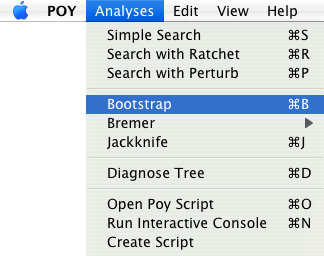
\includegraphics[width=\textwidth]{figures/Bootstrap_Menu.jpg}
\end{minipage}
\quad
\begin{minipage}[c]{0.48\textwidth}
	   	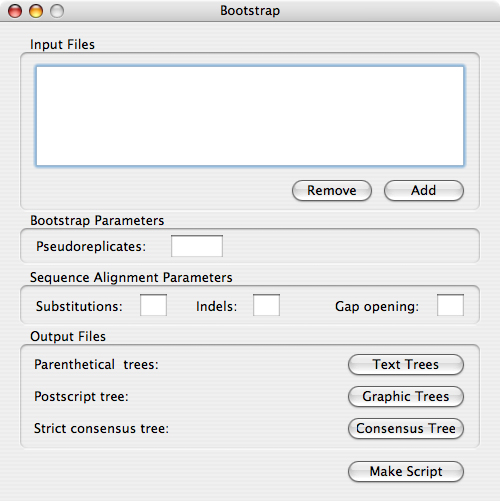
\includegraphics[width=\textwidth]{figures/Bootstrap_Window.jpg}
   	\end{minipage}
\caption{The \emph{Bootstrap} window. Selecting \emph{Bootstrap} from the \emph{Analysis} menu (left) and viewing the \emph{Bootstrap} window options (right).}
\label{fig:bootstrap}
\end{figure}

\subsubsection{Bremer}

The \emph{Bremer} window is divided in two windows: the \emph{Search for Bremer} window, that specifies the Bremer support calculation parameters, and the \emph{Report Bremer} window to format the output of the results. 

\paragraph{Search for Bremer}

\begin{figure}[htpb]
    \begin{center}
        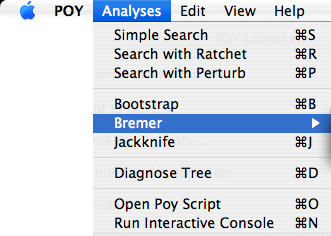
\includegraphics[width=0.65\textwidth]{figures/SearchForBremer_Menu.jpg}
    \end{center}
    \caption{ Selecting the \emph{Bremer} windows from the \emph{Analysis} menu.}
    \label{fig:search_for_bermer_menu}
\end{figure}

\begin{figure}
\centering
\begin{minipage}[c]{0.48\textwidth}
   		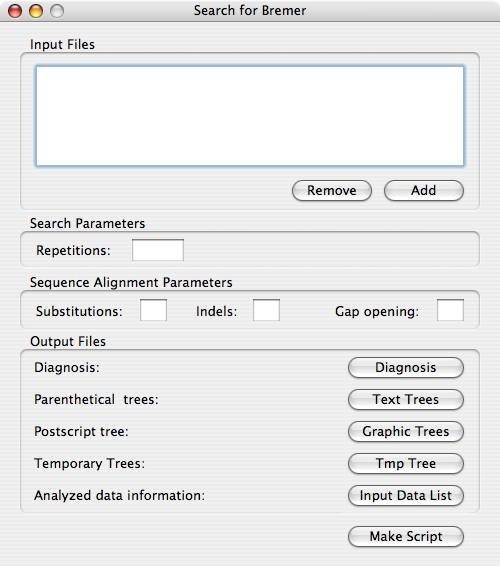
\includegraphics[width=\textwidth]{figures/SearchForBremer_Window.jpg}
\end{minipage}
\quad
\begin{minipage}[c]{0.48\textwidth}
	   	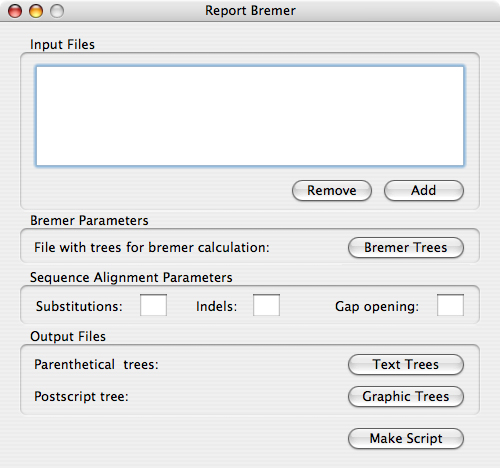
\includegraphics[width=\textwidth]{figures/ReportBremer_Window.jpg}
   	\end{minipage}
\caption{Viewing the options of the \emph{Search for Bremer} (left) and the \emph{Report Bremer}(right) windows.}
\label{fig:search_report_bremer}
\end{figure}

The script produced in this window collects trees visited during a search. This
search can take a long time, as all the tree search heuristics are turned off,
with the goal of sampling a wide variation of trees, and guarantee that all
clades have Bremer support values. 

In addition to the standard four sections defined for the \emph{Simple Search} window,
not that one of the output files is the \emph{Temporary Trees} file, which will
contain \emph{all the information required to produce the bremer support tree
results in the Report Bremer Window}. Make sure that you pick a file that you
will not destroy for this output.

If it takes \poy too long to finish searching for Bremer, the search can be interrupted and the intermediate results stored in the \emph{Temporary Trees} file (however at the risk that that bremer support values can be inflated). The trees from the \emph{Temporary Trees} file can then be reported using the \emph{Report Bremer} window.

\paragraph{Report Bremer}
The script produced in this window takes the ``Temporary
Trees'' file generated in the Search for Bremer window in the ``File with trees for
bremer calculation'' field. 

\subsubsection{Jackknife}

The \emph{Jackknife} window specifies parameters for estimating the
Jackknife support values. The window consists of the same
four sections as the \emph{Simple Search} window except for
\emph{Jackknife Parameters} that has two fields, \emph{Pseudoreplicates}
and \emph{Remove}.

\begin{figure}
\centering
\begin{minipage}[c]{0.48\textwidth}
   		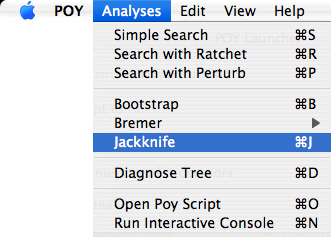
\includegraphics[width=\textwidth]{figures/Jackknife_Menu.jpg}
\end{minipage}
\quad
\begin{minipage}[c]{0.48\textwidth}
	   	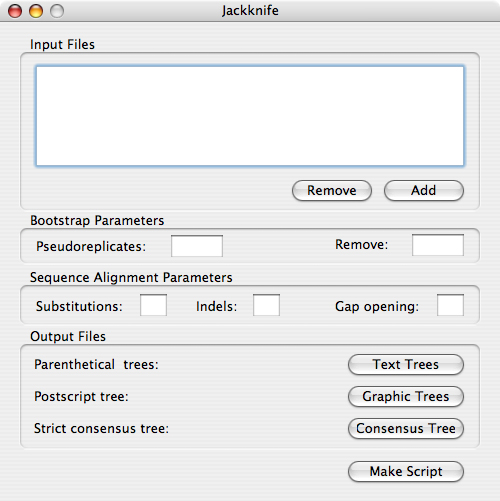
\includegraphics[width=\textwidth]{figures/Jackknife_Window.jpg}
   	\end{minipage}
\caption{The \emph{Jackknife} window. Selecting \emph{Jackknife} from the \emph{Analysis} menu (left) and viewing the \emph{Jackknife} window options (right).}
\label{fig:jackknife}
\end{figure}

\begin{description}
    \item[Pseudoreplicates] Specifies the number of resampling iterations.
    \item[Remove] Specifies the percentage of characters being deleted during a pseudoreplicate.
\end{description}

\subsubsection{Open POY Script}

Selecting \emph{Open POY Script} displays the \emph{POY Launcher}
window, the function of which is described above.

\begin{figure}[htpb]
    \begin{center}
        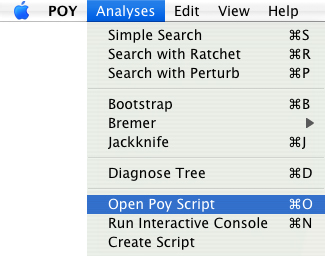
\includegraphics[width=0.5\textwidth]{figures/OpenPoyScript_Menu.jpg}
    \end{center}
    \caption{Open a POY script}
    \label{fig:open_poy_script}
\end{figure}

\subsubsection{Run Interactive Console}

Selecting \emph{Run Interactive Console} opens the ncurses interface
that enables the user to run the analysis interactively by entering
\poy commands directly via the command-line \emph{Interactive
Console}. Note that the interactive console \emph{does not run in parallel.}

\begin{figure}[htpb]
    \begin{center}
        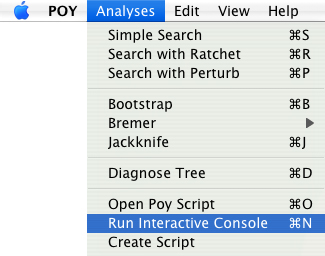
\includegraphics[width=0.5\textwidth]{figures/RunInteractive_Menu.jpg}
    \end{center}
    \caption{Run POY in the interactive console}
    \label{fig:open_poy_script}
\end{figure}
Selecting \emph{Run Interactive Console} opens the ncurses interface
that enables the user to run the analysis interactively by entering
\poy commands directly via the command-line \emph{Interactive
Console}. Note that the interactive console \emph{does not run in parallel.}

\subsection{The \emph{View} menu}

The \emph{View} menu contains selections for the \emph{Results} and \emph{Status} windows.

\subsubsection{The \emph{Results} and \emph{Status} windows}

\begin{figure}[htpb]
    \begin{center}
        
\includegraphics[width=0.5\textwidth]{figures/View_Menu.jpg}
    \end{center}
    \caption{Opening the Results and Status Windows}
    \label{fig:results_and_status_windows}
\end{figure}
The \emph{Results} and \emph{Status} windows report, as their names
imply, the current results of the analysis and the state of the
search. These windows are not updated automatically and in order
to display the current state of the analysis the user must click
the \emph{Update} buttons in the right lower corner of each window.

\section{\poy Interactive Console}

\emph{POY Interactive Console} provides a command line-based environment with enhanced ability to display the results and the state of the analysis. Using the console requires familiarity with \poy commands, their arguments, and the conventions of \poy scripting (which are discussed the \emph{POY Commands} chapter). The console has the same appearance regardless of the operation system under which \poy is run (except under parallel environment settings; see below). It has four windows: \emph{POY Output}, \emph{Interactive Console}, \emph{State of Stored Search}, and \emph{Current Job} (Figure \ref{fig:figinterface}).

\begin{figure}[htbp]
   \centering
   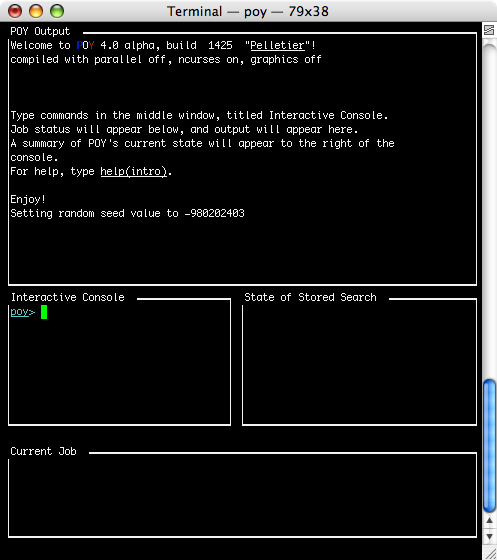
\includegraphics[width=0.7\textwidth]{figures/figinterface.jpg}
   \caption{\poy interface displayed in the Terminal window prior to analysis. Note the cursor at the \poy prompt in the \emph{Interactive Console} and that the \emph{State of Stored Search} and \emph{Current Job} windows are empty.}
   \label{fig:figinterface}
\end{figure}

\begin{description}
\item[POY Output window] displays the status of the imported data, outputs the results of the phylogenetic analyses (such as trees, character diagnoses, and implied alignments), reports errors, and displays descriptions of \poy commands. By default, \poy reports the list of imported data and generates error messages. Other outputs, however, must be requested using the \commandstyle{report()} command.
\item[Interactive Console]  is used to instruct \poy to import data, specify the kinds of analysis to be performed, and to request the desired output interactively by typing \poy commands at the \poy prompt (\texttt{poy$>$}). The commands are executed by hitting the Return key. The commands can be executed one at a time or entered sequentially until the Return key is pressed. (See Section~\ref{commands} on the structure and syntax of \poy commands.) Separating commands by spaces is optional but increases legibility. Alternatively, a file containing the list of commands (\poy script, see below) can also be imported and executed at the prompt in the Interactive Console.
\item[State of Stored Search]  displays the time (in seconds) elapsed since the initiation of the current operation. This window also reports the number of trees currently in memory and provides the range of their costs.
\item[Current Job] describes the currently running operation. When the operation is completed, the window is blank.
\end{description} 

\begin{figure}[htbp]
   \centering
   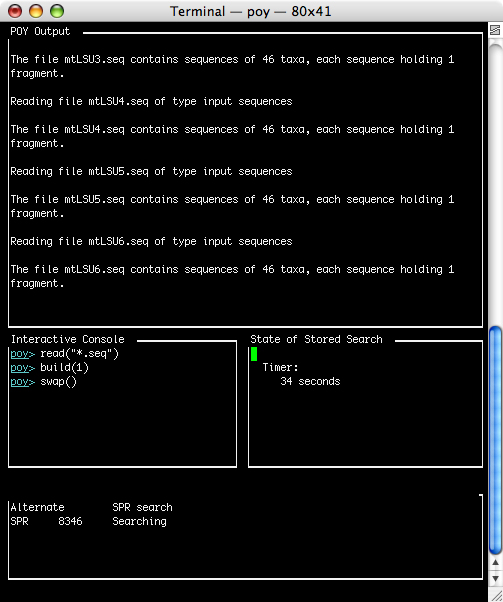
\includegraphics[width=0.7\textwidth]{figures/figprocess.jpg}
   \caption{\poy interface during a process. The \emph{POY Output} window displays (by default) the information on the input datafiles. The \emph{Interactive Console} lists the commands that have been consecutively executed. The \emph{Current Job} window shows the state of the current operation and the current tree score. The \emph{State of Stored Search} shows the time elapsed  since the last command, \commandstyle{swap}, was initiated.}
   \label{fig:figprocess}
\end{figure}

This \poy interface is not available for parallel environments. Once the program is called, \poy commands can be executed interactively or scripts can be submitted as when using the \emph{Interactive Console}. By default, the \poy will print the output on screen (the same output that is reported in \emph{POY Output} under non-parallelized setting).

\subsection{Starting a \poy session using the \emph{Interactive Console}}

\begin{flushleft}
	\begin{minipage}[c]{0.075\textwidth}
	   	
\includegraphics[width=\textwidth]{figures/figLogoWindows.jpg}
	\end{minipage}
	\quad
	\begin{minipage}[t]{0.89\textwidth}
		\subsubsection{Windows}
	\end{minipage}
			\begin{itemize}
                \item{Start$>$All Programs$>$POY$>$POY Interactive Console}
			\end{itemize}

	\begin{minipage}[c]{0.075\textwidth}
   		
\includegraphics[width=\textwidth]{figures/figLogoMac.jpg}
	\end{minipage}%
	\quad
	\begin{minipage}[t]{0.89\textwidth}
	   	\subsubsection{Mac OSX}
	\end{minipage}
			\begin{itemize}
				\item {Double-click \poy application icon to start the program.}
				\item {Select \emph{Run Interactive Console} from the
				\emph{Analyses} menu.}
			\end{itemize}		

	\begin{minipage}[c]{0.075\textwidth}
   		
\includegraphics[width=\textwidth]{figures/figLogoLinux.jpg}
	\end{minipage}%
	\quad
	\begin{minipage}[t]{0.89\textwidth}
	   	\subsubsection{Linux}
	\end{minipage}
    Add \texttt{/opt/poy4/Resources/} to your \texttt{PATH} and then simply run
    \texttt{ncurses\_poy} from a terminal.
\end{flushleft}

\begin{figure}[htbp]
   \centering
   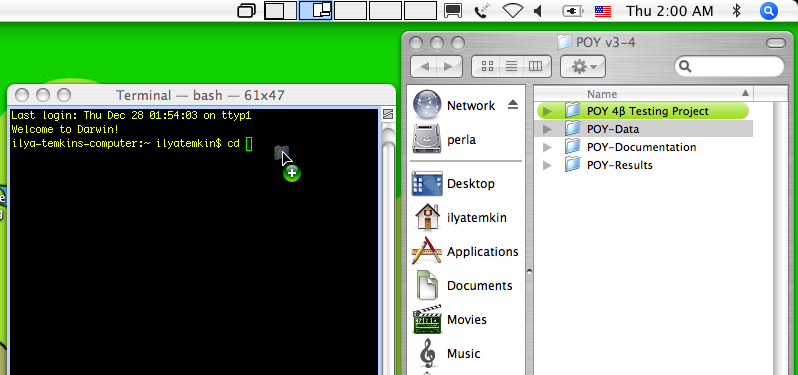
\includegraphics[width=0.7\textwidth]{figures/figprelim1.jpg}
   \caption{Specifying the location of datafiles. The folder \texttt{POY-Data} is dragged from the \texttt{POY v3-4} folder directly in the Terminal window.}
   \label{fig:figprelim1}
\end{figure}

\begin{figure}[htbp]
   \centering
   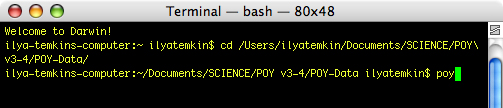
\includegraphics[width=0.7\textwidth]{figures/figprelim2.jpg}
   \caption{Starting \poy. At the folder containing datafiles, entering \texttt{poy} starts a \poy session.}
   \label{fig:figprelim2}
\end{figure}

\subsection{Entering commands}
The \emph{Interactive Console} is the only part of the interface that allows communication with \poy; that is where commands and scripts are executed. Once the \poy interface is called, the cursor appears in the \emph{Interactive Console} and \poy is ready to accept commands. \poy interface does not support using the mouse and, as true for most command-line applications, the cursor can be moved using the left and right arrow keys, and the Backspace (in Windows) or Delete (in Mac) keys are used to erase individual characters to the left of the current cursor position. To eliminate the need of retyping commands anew during a \poy session, keyboard shortcuts can be used: Control-P (``previous'') and Control-N (``next'') will scroll through the commands entered during the session.

\subsection{Browsing the output}
As more output is reported in the \emph{POY Output} window, only the most recent reports will be seen in the window. Using the Up and Down keys allows to scroll up and down the \emph{POY Output} window to see the welcome line, and previously printed reports and help descriptions. Pressing Up and Down keys automatically places the cursor in the lower left corner of the \emph{POY Output} window indicating that you are interacting with that window. It is important to know that only 1000 lines are stored in the memory and the output that was reported before that will not be accessible by scrolling. If it is desired to keep the entire output or specific items in the output, the log can be created (using the command \poycommand{set()}, see~\ccross{log}) or specific outputs can be redirected to files (see~\ccross{report}).

\subsection{Switching between the windows}
To return to the \emph{Interactive Console} start typing and the cursor will automatically be placed back at the \poy prompt. When an operation is in progress (which is shown in the \emph{Current Job} window), the cursor stays in the upper left corner of the \emph{State of Current Search} window, and switching between the \emph{Interactive Console} and the \emph{POY Output} window is disabled. There are no user interactions with the \emph{Current Job} and \emph{State of the State of Current Search}.

\subsection{Interrupting a process}
To interrupt a process, press Control-C. By default, an error, \texttt{Error:}\\ \texttt{Interrupted}, is reported in the \emph{POY Output} window. The program does not close, however, and a new command can be entered. This command does not close the program, it only stops the last process that was running keeping in memory all the data and the results of the operation executed last. New commands can subsequently be entered.

\subsection{Reporting errors}
\poy reports errors in several ways. If there is an error pertaining to wrong syntax (such as a typo in a command name), \poy will indicate the location of an error by underlining the problematic part of the input with ``\texttt{\^}'' in the \emph{Interactive Console} (Figure~\ref{fig:errors}). \poy will also automatically display in the \emph{POY Output} window the description of the command, its syntax, and examples of its usage. As explained above, the Up and Down keys can be used to scroll through the output and determine the source of the error. Certain kinds of errors will be reported explicitly (Figure~\ref{fig:errors}).

\begin{figure}
\centering
\begin{minipage}[c]{0.48\textwidth}
   		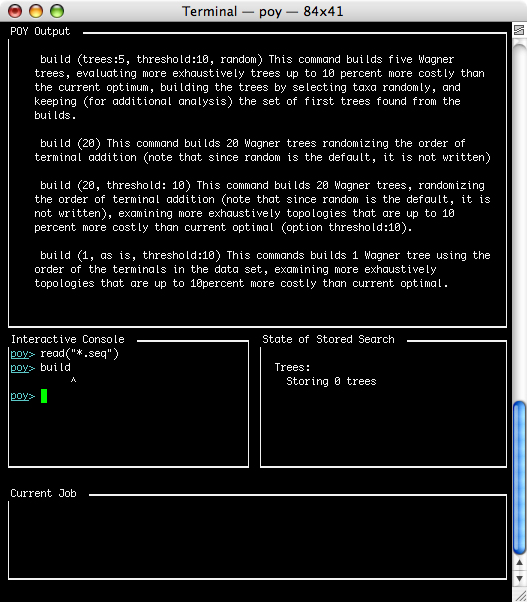
\includegraphics[width=\textwidth]{figures/figerror1.jpg}
\end{minipage}%
\quad
\begin{minipage}[c]{0.48\textwidth}
	   	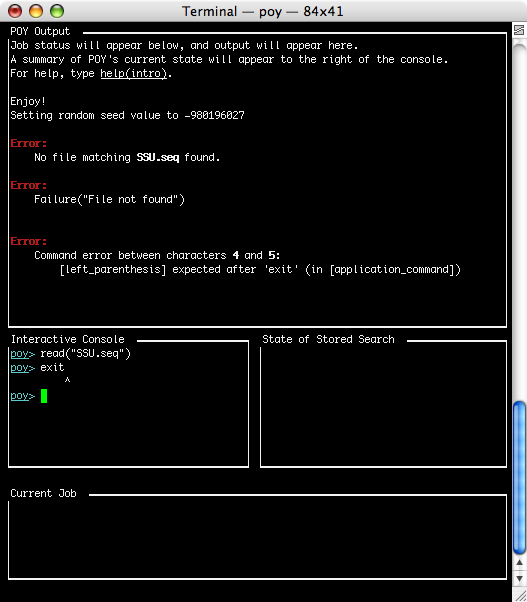
\includegraphics[width=\textwidth]{figures/figerror2.jpg}
   	\end{minipage}
	
\caption{Displaying errors. \poy displays error messages in several ways. In the example in the left panel, the command \commandstyle{build} was entered without parentheses, which is required for a  valid \poy command syntax; The exact place of the error is marked by ``\texttt{\^}'', in this case  following the \commandstyle{build} commands. Examples of the proper usage of the command are automatically displayed in the \emph{POY Output}. In other cases (right panel), error messages are explicitly reported in the \emph{POY Output} window. The first and second error messages indicate that the datafile \texttt{SSU.seq} is not present, which could have been caused either by a mistake in the name of the file, missing file, or the location of the file in a directory, other than the one specified prior to starting the \poy session. The third error message indicates that the valid syntax of \commandstyle{exit} requires the parentheses following the command name (also shown by ``\texttt{\^}'' in  the \emph{Interactive Console}).}
\label{fig:errors}
\end{figure}

\subsection{Exiting}
To finish a \poy session, enter command \commandstyle{exit()} (Figure~\ref{fig:exithelp}) or \commandstyle{quit()}. This will close the \poy interface and resume the Terminal window (Mac) or the Command Prompt window (Windows).

\begin{figure}[]
    \begin{center}
        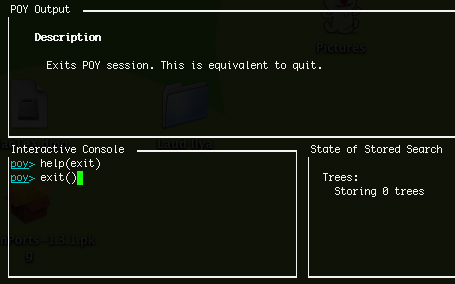
\includegraphics[width=0.5\textwidth]{figures/exithelp.jpg}
    \end{center}
    \caption{Exiting \poy}
    \label{fig:exithelp}
\end{figure}

\section{Obtaining help} \label{sec:help}
Instructions to run \poy, command descriptions, and the theory behind \poy can be obtained from a variety of sources.
\begin{description}
\item[POY] contains a help file that can be accessed by entering \commandstyle{help()} at \poy prompt in the \emph{POY Output} window. This file contains descriptions and examples of all currently implemented \poy commands. Up and down arrows allow to scroll through the file. To obtain help on a particular command, the name of the command must be specified in the parentheses following \commandstyle{help()}. For example, to learn about the command \commandstyle{exit}, type \commandstyle{help(exit)}. Help will appear in the upper window, as shown in Figure~\ref{fig:exithelp}.
\item[Quick Start and Program Documentation] is a comprehensive and detailed manual on all the aspects of using \poy, from installation to outputting and visualizing the results. It includes a \emph{Quick Start}, a \poy command reference, practical guides and tutorials that make the program immediately accessible for beginners and provide in-depth information for experienced users. The documentation in PDF format can be accessed from the \emph{Help} menu of the graphical user interface or downloaded separately from \poy web site at
\begin{center}
\texttt{http://research.amnh.org/scicomp/projects/poy.php}
\end{center}
\item[POY Book] (Wheeler et al., 2006 \emph{Dynamic Homology and Phylogenetic Systematics: A Unified Approach Using POY}) provides a review of the theory behind \poy, and contains formal descriptions of many algorithms implemented in the program and the descriptions of commands of the earlier version, \texttt{POY3}.
\item[POY4 Mail Group] is an Internet-based forum for discussing all issues related to \poy and provides the best way to communicate with \poy developers on specific issues (see \emph{WWW resources} below). The website is located at \texttt{http://groups.google.com/group/poy4}.
\begin{figure}[htbp]
   \centering
   
\includegraphics[width=0.23\textwidth]{figures/figPOYBook.jpg}
   \caption{The \poy Book.}
   \label{fig:figprocess}
\end{figure}
\end{description}

\section{WWW resources}
\poy is an ongoing project and new versions are being continuously developed to include new procedures, improve performance, and eliminate reported bugs. Therefore, it is imperative to keep up with the program's development and check regularly for updates. There are several Internet-based resources that offer this information, and, additionally, provide a forum for discussing specific issues using \poy, and present an efficient way to communicate with \poy developers regarding any technical difficulties, reporting bugs, and obtaining help.

\begin{description}
\item[POY4 Web Site] has downloadable compressed files of \poy binaries, source code, and documentation in PDF format. It also provides a links to the \emph{POY Mail Group}. The website is hosted by AMNH Computational Sciences at 
\begin{center}
\texttt{http://research.amnh.org/scicomp/projects/poy.php}
\end{center}
\item[POY4 Mail Group] informs registered users via email of new developments, such as new versions and updates. It also provides a way for reporting bugs and other problems with \poy and its documentation, as well as an additional resource for obtaining help on specific issues. In addition, it allows users to receive and respond to each other's questions thus providing an open forum to  discuss the methods and applications of \poy. The users who choose not to register, will have access to the archives of the postings but will not be able to either submit or receive emails from other users and \poy developers. The \emph{POY4 Mail Group} is hosted  by Google at
	\begin{center}
	\texttt{http://groups.google.com/group/poy4}
	\end{center}
	
%	\item[Mantis] is a bug tracking system. It provides an extremely efficient, automated way to describe, sort, and prioritize reported bugs and other technical issues concerning both the program and the documentation. Users are strongly encouraged to establish an account and to submit their reports using \emph{Mantis}. Streamlining the troubleshooting process benefits the users in the long run as it provides the means to produce a new and improved version of \poy much more efficiently and within a shorter period of time. \emph{Mantis} is hosted by the AMNH at
%	\begin{center}
%	\texttt{https://research.amnh.org/mantis/login\_page.php}
%	\end{center}
\end{description}

\section{Using \poy}

This section will help you get started using \poy and will prepare you for the
more extensive, technical descriptions in the next chapter, \emph{\poy Commands}. Now that you are acquainted with the program's interface, learned how to initiate, and exit or interrupt) a \poy session, and how to obtain help, you are well prepared to run your first analysis. This chapter will teach
you how to read (import) datafiles, check the data you are analyzing, generate
a set of initial trees, do basic branch swapping to find a local optimum, and, finally, produce
and visualize the resultant trees, their strict consensus, and generate support values.

For the purpose of this exercise, three datalfiles are used. These sample files can be downloaded from \\
\texttt{http://research.amnh.org/scicomp/projects/poy.php}:

\begin{itemize}
	\item {\texttt{18s.fas} contains unaligned DNA sequence data for a single locus (partial 18S ribosomal DNA) in FASTA format.}
	\item {\texttt{28s.fas} contains unaligned DNA sequence data for a single locus (partial 28S ribosomal DNA) in FASTA format.}
	\item {\texttt{morpho.ss} contains a morphological data matrix in Hennig86 format.}
\end{itemize}

Once \poy has been launched and the interface (Figure~\ref{fig:figinterface}) had appeared on the screen, the data can be imported and the analysis can proceed. As you follow the instructions, you are encouraged to consult the help file by using the command \commandstyle{help} (see Section~\ref{sec:help} to learn more about \poy commands and their arguments).

\subsection{Importing data} \label{sec:import}

The basic command to input data in \poy is \commandstyle{read()}, which includes the list of files (in quatation marks and separated by commas) enclosed in parentheses. Suppose that we would like to simultaneously analyze morphological and molecular datasets, contained in separate datafiles, \texttt{morpho.ss} and \texttt{28s.fas}, respectively. We can issue a pair of \commandstyle{read()} commands (Figure~\ref{fig:readingexample}):
\begin{quote}
        \commandstyle{read("morpho.ss")}\\
        \commandstyle{read("28s.fas")}
\end{quote}

\begin{figure}
    \begin{center}
        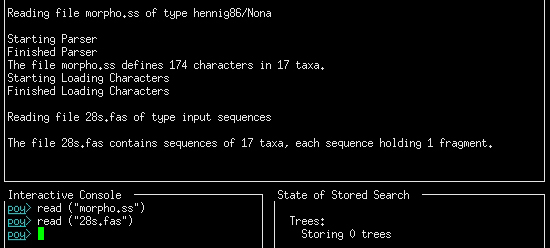
\includegraphics[width=0.6\textwidth]{figures/reading_example.jpg}
    \end{center}
    \caption{Importing datafiles using the \emph{Interactive Console}. Two consecutive \commandstyle{read} commands import both the morphological datafile in Hennig86 format (\texttt{morpho.ss}), and the molecular datafile in Fasta format (\texttt{28s.fas}) . Note that \poy automatically reports  in the \emph{POY Output} window the names and types of files that have been imported.}
    \label{fig:readingexample}
\end{figure}

The syntax of \commandstyle{read} is not unique; in fact, every command in \poyv contains two elements: the name of the command (e.g. \commandstyle{read}), followed by the list of arguments 
separated by commas and enclosed in parentheses. Typically, the arguments of the command \commandstyle{read()} are names of datafiles, each being enclosed in double quotes (as shown in the example above). Eventhough arguments there might be only one argument or it might be absent or omitted in some commands, parentheses (e.g.\poycommand{read()}) always follow the command name. An exhaustive discussion of \poy command structure and detailed descriptions of all commands with examples of their usage are provided in the \emph{POY Commands Reference} document.

Most of the time users are interested in importing multiple datafiles to analyze on the entire dataset. In this case, multiple datafiles can be specified as arguments for a single command. For example, importing both files, \texttt{morpho.ss} and \texttt{28s.fas}, can be written more succinctly:
\commandstyle{read("morpho.ss", "28s.fas")}. This is equivalent to sequentially importing each file at a time as was shown previously (Figures ~\ref{fig:readingexample} and \ref{fig:reading_example2}).

Figure~\ref{fig:readingexample} also illustrates an important feature that makes \poy
different from many other phylogenetic analysis programs: every
time a file is imported during a \poy session, the input data is \emph{added} to the current data in memory, it \emph{does not replace it}. This allows additional analytical flexibility. For example, if only morphological data are read and trees are built based on these data alone, a subsequently imported molecular character dataset will be used in conjunction with the previously imported morphological data in subsequent operations, despite the fact that the trees were generated only from morphological data (Figure~\ref{fig:reading_example2}):

\begin{quote}
\commandstyle{read("morpho.ss")}\\
\commandstyle{build()}\\
\commandstyle{read("28s.fas")}\\
\commandstyle{rediagnose()}\\
\commandstyle{swap()}
\end{quote}

It must be noted that if the number of terminals differs among datafiles, only the data that corresponds to the terminals used to generate the trees (from the morphological datafile in our example) are used; the rest of the character data are ignored.

Also, because \poy appends trees and data in memory, it is a good practice to empty the memory when starting a new analysis using use the \commandstyle{wipe()} command (see also \commandstyle{clear\_memory()}).

\begin{figure}[]
    \begin{center}
        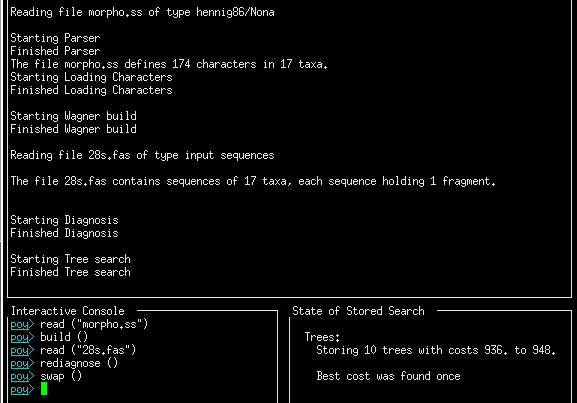
\includegraphics[width=0.6\textwidth]{figures/reading_example2.jpg}
    \end{center}
    \caption{Building trees with morphological data only but continuing analysis using combined morphological and molecular data. This example shows how we can add data to the analysis incrementally by loading files at different points in the search. First, the morphological data are imported from \texttt{morpho.ss} file using \poycommand{read()} the and trees are built based on these data. Then molecular data from the \texttt{28s.fas} file are loaded into memory in addition to previously imported morphological data. Finally, subsequent analyses, \commandstyle{rediagnose()} and \commandstyle{swap()}, are conducted using the data in memory, that is the trees based on morphological data, and both morphological and molecular character sets.}
    \label{fig:reading_example2}
\end{figure}

Valid input files include nucleotide and amino acid sequence files in many formats,
and morphological data in Hennig 86 format. For information on specific formats supported by \poy and other types of input files see \commandstyle{help(read)}.

\subsection{Inspecting data}

Once a dataset (or multiple datasets) is imported, \poy automatically reports a brief description of contents for each loaded file in the \emph{POY Output} window as shown in Figure ~\ref{fig:readingexample}. However, it may be desirable to inspect the imported data in greater detail to ensure that the format and contents of the files has been interpreted correctly. This practice allows to avoid common errors, such as misspelled terminal names, which may result in bogus results, produce error messages, and aborted jobs.

The basic command for outputting information is \commandstyle{report()}. One of its arguments, \commandstyle{data}, outputs a set of tables showing the list of terminals, the number and type of characters, the list of files that have been imported so far, and the lists of terminals and characters excluded from the analysis. For example, to produce such report of the same datafiles that were used in the previous example (\texttt{morpho.ss} and \texttt{28s.fas}), we import the data and execute \commandstyle{report(data)}:
\begin{quote}
    \commandstyle{read("morpho.ss","28s.fas")}\\
    \commandstyle{report(data)}
\end{quote}
This will generate an extensive, detailed output, partial views of which are shown in Figure ~\ref{fig:reportdata}. Obviously, the entire report will not be visible in the \emph{POY Output} window. Therefore, the Up and Down arrow keys should be used to scroll through it.

\begin{figure}
\centering
\begin{minipage}[c]{0.52\textwidth}
   		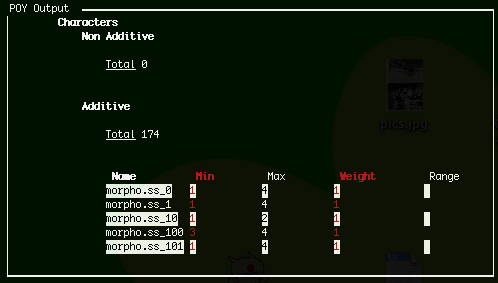
\includegraphics[width=\textwidth]{figures/report2.jpg}
\end{minipage}
\quad
\begin{minipage}[c]{0.44\textwidth}
	   	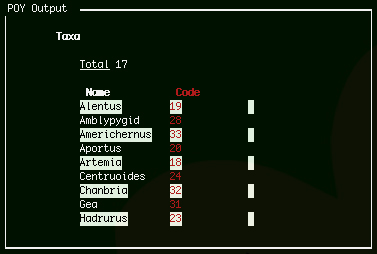
\includegraphics[width=\textwidth]{figures/report3.jpg}
   	\end{minipage}
\caption{Inspecting imported data. The figure shows segments of a data report generated by \commandstyle{report(data)}. The left and right panels demonstrate a typical table output the character and terminal data respectively.}
\label{fig:reportdata}
\end{figure}

In this example, all the imported data is analyzed and, therefore, the report fields that list excluded data will appear empty in the report. One can, however, exclude specific characters or terminals from the analysis using additional commands (see \commandstyle{select()}).

By default, \poy reports the results of executed commands in the \emph{POY Output} window. However, the same output can be redirected to a file simply by adding the name of the output file in the list of argument of the command \commandstyle{report()} \emph{before} the argument that specified the type of the requested report (in this case \commandstyle{data}). For instance, if we would like to output into the file ``data\_analyzed.txt'', we would write \commandstyle{report("data\_analyzed.txt", data)}.

Another useful argument of \commandstyle{report} is \commandstyle{cross\_references}. It displays which terminals are present or absent in each one of the imported files, providing a comprehensive visual overview of the missing data. Building on the previous example, such output can be generated by the following sequence of commands:
\begin{quote}
    \commandstyle{read("morpho.ss", "28s.fas")}\\
    \commandstyle{report(cross\_references)}
\end{quote}

\begin{figure}[]
    \begin{center}
        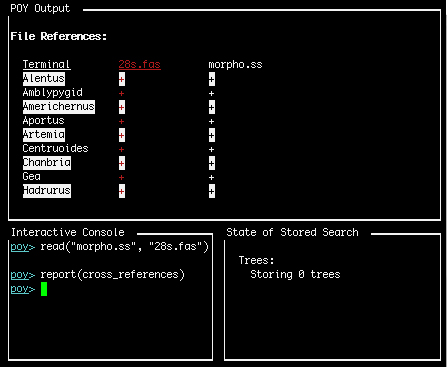
\includegraphics[width=0.6\textwidth]{figures/crossref.jpg}
    \end{center}
    \caption{Visualizing missing data. The command \commandstyle{cross\_references} displays a table showing whether a given terminal (in the left column) is present (``+'') or absent (``-'') in each datifie. In this example, the data for all the the taxa listed in the \emph{POY Output} window are present both datafiles, \texttt{morpho.ss} and \texttt{28s.fas}.}
    \label{fig:crossref}
\end{figure}

A typical output of \commandstyle{cross\_references} command is shown in Figure ~\ref{fig:crossref}.

\subsection{Building initial trees}

The command to build trees is \commandstyle{build} (already been mentioned in Section~\ref{sec:import}). After importing \texttt{morpho.ss} and \texttt{28s.fas}, executing the command \commandstyle{build()} without specifying any arguments will generate 10 Wagner trees by random addition sequence (the default setting of the command). Make sure that if you plan to build trees based on other data you have to purge the memory first by using \commandstyle{wipe()} command
Many \poy commands operate under default settings when executed without arguments. (To learn what the default settings are for a particular command, use either \commandstyle{help()} command with the command name of interest inserted in parentheses or consult the \emph{POY Commands Reference}; see Section~\ref{sec:help}.) If you would like to build more trees, 100 for instance, an argument \commandstyle{trees} followed by a colon (``:'') and an integer specifying the number of trees must be included in the argument list of the \commandstyle{build} command: \commandstyle{build(trees:100)}. This command has a shortcut that omits the argument \commandstyle{trees}; therefore, \commandstyle{build(trees:100)} is equivalent to \commandstyle{build(100)}. As defaults, the shortcuts are fully described in the \emph{POY Commands Reference}. The entire sequence of commands minimally required to import the data and build 100 trees is the following:

\begin{quote}
 	\commandstyle{read("morpho.ss","28s.fas")}\\
 	\commandstyle{build(100)}
\end{quote}

As the tree building advances, the \emph{Current Job} window displays the current status of the operation (Figure~\ref{fig:building}). It shows how many Wagner builds have been performed out of the total number requested, the number of terminals added in the current build, the cost of a current tree (recalculated after each terminal addition), and the estimated time (in seconds) for the completion of all the builds. When all the trees are generated, the \emph{State of Stored Search} window displays the range of tree costs (the best and worst costs), the number of trees stored in memory, and the number of trees with the best cost.

\begin{figure}
\centering
\begin{minipage}[c]{0.507\textwidth}
   		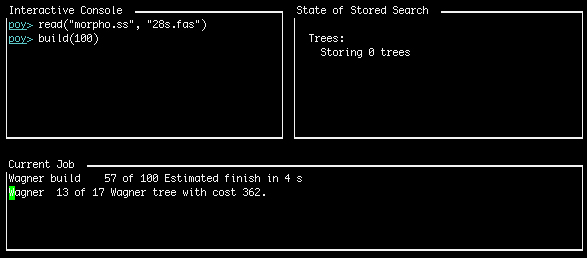
\includegraphics[width=\textwidth]{figures/building1.jpg}
\end{minipage}%
\quad
\begin{minipage}[c]{0.453\textwidth}
	   	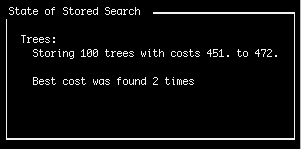
\includegraphics[width=\textwidth]{figures/building2.jpg}
   	\end{minipage}
\caption{Generating Wagner trees. During the process of tree building (left panel), the \emph{Current Job} window displays how many builds have been performed so far (\texttt{57 of 100}), the number of terminals added in the current build (\texttt{13 of 17}), a cost of a current tree recalculated after each terminal addition (\texttt{362}), and the estimated time (in seconds) for the completion of the operation (\texttt{4 s}). Because the process is not complete, the \emph{State of Stored Search} window contains no trees. Once tree building is finished, the \emph{State of Stored Search} window displays the best (\texttt{451}) and worst (\texttt{472}) costs, the number of trees stored in memory (\texttt{100}), and the number of trees with the best cost (\texttt{2}).} 
\label{fig:building}
\end{figure}

\subsection{Performing a local search}

Now, that the trees have been generated and stored in memory, a local search can be performed to refine and improve the initial trees by examining additional topologies of potentially better cost.  The command \commandstyle{swap()} implements an efficient strategy by performing SPR and TBR branch swapping iteratively. As with other commands, the arguments of \commandstyle{swap()} allow customization of the performance of the command. In case of \commandstyle{swap()}, additional options specify which algorithms are used in swapping and restrict swapping to certain sections of trees. In the following example, branch swapping is performed under the default settings on each of the 100 trees build in the previous step:

\begin{quote}
 	\commandstyle{read("morpho.ss","28s.fas")}\\
 	\commandstyle{build(100)}\\
	\commandstyle{swap()}
\end{quote}

Branch swapping is performed sequentially on all trees stored in memory. During swapping, the \emph{Current Job} window reports the number of a tree that is currently being analyzed, the method of branch swapping, the specific routine being currently performed, and the cost of the current tree (Figure~\ref{fig:swapping}). When the process is complete, the \emph{State of Stored Search} window displays the range of tree costs (the best and worst costs), the number of trees stored in memory, and the number of trees of the best cost (Figure~\ref{fig:swapping}). Note that the local search had reduced the costs of the initial best (from 451 to 446) and narrowed the range of tree costs.

\begin{figure}
\centering
\begin{minipage}[c]{0.49\textwidth}
   		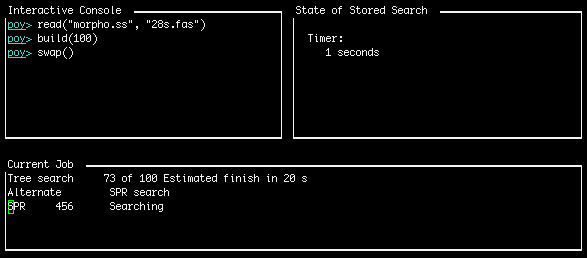
\includegraphics[width=\textwidth]{figures/swap1.jpg}
\end{minipage}
\quad
\begin{minipage}[c]{0.453\textwidth}
	   	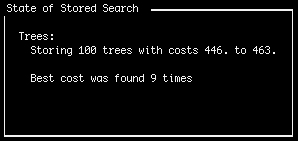
\includegraphics[width=\textwidth]{figures/swap2.jpg}
   	\end{minipage}
\caption{Performing a local search. When searching (left panel), the \emph{Current Job} window reports the number of the tree that is currently being analyzed (\texttt{73 of 100}), a method of branch swapping (\texttt{Alternate}), a function being currently performed (\texttt{SPR search}), and a cost of the current tree (\texttt{456}). When the searching is finished (right panel), the \emph{State of Stored Search} window displays the best (\texttt{446}) and worst (\texttt{463}) costs, the number of trees stored in memory (\texttt{100}), and the number of trees of the best cost (\texttt{9}) recovered from independent tree builds. Note these trees may not necessarily have unique topology.} 
\label{fig:swapping}
\end{figure}

Using different combinations of the arguments of \commandstyle{swap()} allows to design a  large number of search strategies of different levels of complexity. Some simple options allow the choice between SPR and TBR. More complex strategies allow keeping a specific number of best trees per single initial tree (generated during the building step). For example, the command \commandstyle{swap(trees:10)} will keep up to 10 best trees generated during branch swapping on a single initial tree. Consequently, if 100 trees were built initially, this command will produce 1,000 trees. The argument \commandstyle{threshold} allows the retention of suboptimal trees within a specified percent of cost difference from the current best tree. For example, \commandstyle{swap(trees:10, threshold:10)}. Other options provide the means to sample trees as they are evaluated, timeout after certain number of seconds, transform the cost regime, and other perform other functions in conjunction with other \poy commands.

%\section{Manipulating characters}

%One of the fundamental steps in phylogenetic analysis is the experimentation
%with cost regimes if using Maximum Parsimony, and models if using Maximum
%Likelihood. \poyv offers the \commandstyle{transform} command to modify the
%characteristics of a particular character as loaded.

%By default, a molecular sequence loaded is assigned with insertion and deletion cost 2 and
%substitution cost 1. In \poyv we can assign different cost regimes to each
%fragment independently. For example, suppose that we would like to load the
%characters stored in the FASTA files 28s.fas and 18s.fas. Then we would like to
%change their cost regime to 1 for indels and 1 for substitutions, and then
%perform a default build and local search. The following commands would do that
%job:

%\begin{lstlisting}
%    (* First read the files *)
%    read ("28s.fas", "18s.fas")

%    (* Now we modify the transformation cost matrix of all the
%    characters *)
%    transform (tcm:(1,1))
%    (* Observe that the argument is tcm, the acronym for transformation
%    cost matrix. *)

%    (* Time to build and swap *)
%    build ()
%    swap ()
%\end{lstlisting}
%Try this example, just as shown in Figure~\ref{fig:transforming}.

%\begin{figure}[]
%    \begin{center}
%        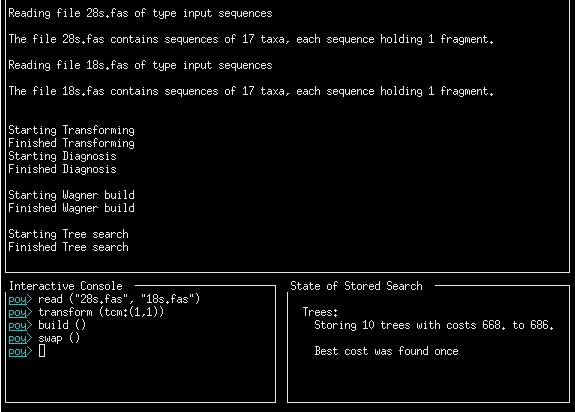
\includegraphics[width=0.6\textwidth]{figures/transforming.jpg}
%    \end{center}
%    \caption{Transforming all the dynamic homology characters in memory to use a
%    transformation cost matrix where insertions, deletions, and substitutions  
%    have cost 1. After reading the data, all the characters are transformed,
%    then we build and swap with that cost regime.}
%    \label{fig:transforming}
%\end{figure}

%However, we might want to analyze the dataset using a different
%cost regime for each one of those two fragments. Say we would like
%to use insertion and deletion cost 3 and substitution cost 1 for
%the 28s fragment, while insertion and deletion and substitution
%cost 1 in the fragment 18s.

%In order to do this, we first check what is the name currently used
%by \poy to refer to each character. We can do this using the
%\commandstyle{report (data)} command that we learned earlier. You
%can see in the list of dynamic homology characters that 28s is
%called 28s\_0 and 18s is called 18s\_0. We can now transform each
%one of them:
%\begin{lstlisting}
%    read ("28s.fas", "18s.fas")

%    (* Now we modify the transformation cost matrix of each character
%    independently *)
%    transform ((names ("18s_0"), tcm:(3,1)))
%    transform ((names ("28s_0"), tcm:(1,1)))

%    build ()
%    swap ()
%    
%\end{lstlisting} The parenthesis might seem a little bit confusing,
%but they provide additional power, we can transform by pairs of
%characters and transformations, in this case, first in those characters
%with name \commandstyle{28s\_0} apply the transformation
%\commandstyle{tcm:(3,1)}, and in those characters with name
%\commandstyle{18s\_0} apply the transformation \commandstyle{tcm:(1,1)}. Why
%using the extra parenthesis to enclose the pair? 
%Just as in read, where we could do several reads in one long command, we can do
%the same with these transforms, so in this case the pair of lines 
%\begin{lstlisting}
%    transform ((names ("18s_0"), tcm:(1,1)))
%    transform ((names ("28s_0"), tcm:(1,1)))
%\end{lstlisting}
%can be written shorter as
%\begin{lstlisting}
%    transform ((names ("18s_0"), tcm:(1,1)),
%        (names ("28s_0"), tcm:(1,1)))
%\end{lstlisting}
%The newline dividing is only here to make the command on screen (or
%paper).  You can leave it or remove it, spaces and newlines are
%ignored.

%There are many more transformations that are allowed in \poyv, for example, if
%the alignments of the 18s fragment are not variable, we can fix it using static
%approximation, in this way, the analysis will go much faster. To do this use
%\begin{lstlisting}
%    transform ((names ("18s_0"), static_approx))
%\end{lstlisting}
%and \poy will choose the shortest tree in memory, produce an implied
%alignment for the fragment 18s\_0, and use it to define a set of static homology
%characters that are equivalent to the alignment cost regime assigned to that
%fragment. Note that after this transformation the command
%\commandstyle{report (data)} will show a set of static homology characters, in
%addition to the (now unique) dynamic homology character 28s\_0. For more
%information see \commandstyle{help (transform)}.

\subsection{Selecting trees}

Having performed the basic steps of importing character data, building initial trees, and conducting a local search, we obtained a set of local optimum trees in memory. Most of the time, a user would like to select only those trees that are optimal and topologically unique and the default setting of the \commandstyle{select()} does exactly that. Adding \commandstyle{select()} to our example of command sequence for the basic analysis 
\begin{quote}
 	\commandstyle{read("morpho.ss","28s.fas")}\\
 	\commandstyle{build(100)}\\
	\commandstyle{swap()}\\
	\commandstyle{select()}
\end{quote}
will select only unique trees of best cost; the remaining trees will be deleted from memory. The \emph{State of Stored Search} window will report the number and the cost of the best tree(s) (Figure~\ref{fig:select}).

\begin{figure}[]
    \begin{center}
        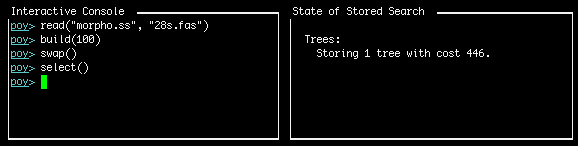
\includegraphics[width=0.6\textwidth]{figures/select.jpg}
    \end{center}
    \caption{Selecting unique best trees. Executing \commandstyle{select()} keeps only unique tees of best cost. The \emph{State of Stored Search} window reports that there is only one unique tree of best cost (\texttt{446}).}
    \label{fig:select}
\end{figure}

\commandstyle{select()} is another multifunctional command the arguments of which are also used to select (include or exclude) specific terminals, characters, and trees.)

Comparing the output reported in the \emph{State of Stored Search} before (Figure~\ref{fig:swapping}) and after (Figure~\ref{fig:select}) executing \commandstyle{select()} shows that swapping on 9 of 100 initial trees produced the trees of best cost (\texttt{446}), but these trees are identical, because only one was retained when filtered using \commandstyle{select()}.

\subsection{Visualizing the results}

There are several ways to visualize results. A quick way to see the tree(s) on screen is to use the command \commandstyle{report(asciitrees)} that will draw a cladogram in the \emph{POY Output} window (Figure~\ref{fig:trees}). The ascii tree can also be reported in a file, if the output file name is specified (in parentheses and separated from the argument \commandstyle{asciitrees} by a comma). However, for reporting trees to a file there are better options. First, the command \commandstyle{report("my\_first\_tree", graphtrees)} will output a cladogram in postscript format (Figure~\ref{fig:trees}) which can be edited using graphics software (such as Adobe Illustrator or Corel Draw). (\poy will also append the ``ps'' extension when generating graphic output to a file.)

\commandstyle{report("my\_first\_trees", trees)} will report the trees in memory to the file \texttt{my\_first\_trees} that can be imported in other programs (such as TNT). Other supported tree tree formats include Newick and Hennig86. \commandstyle{report()} can also generate consensus trees in the graphical (postscript) format when appropriate arguments are specified (for example, \commandstyle{report("strict\_consensus", graphconsensus)}).

\begin{figure}
\centering
\begin{minipage}[c]{0.45\textwidth}
   		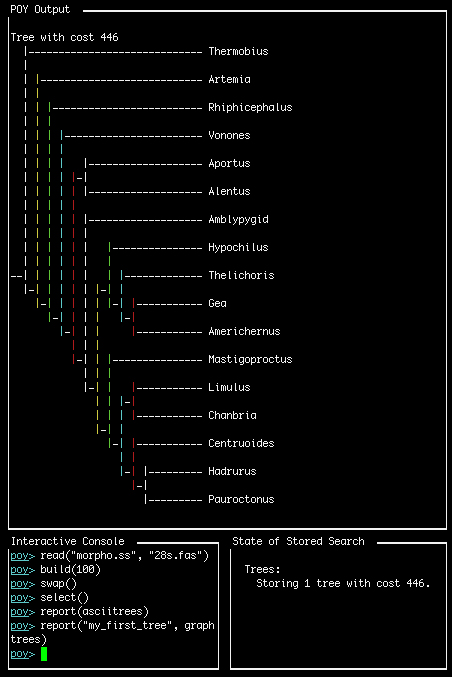
\includegraphics[width=\textwidth]{figures/asciitree.jpg}
\end{minipage}
\quad
\begin{minipage}[c]{0.5\textwidth}
	   	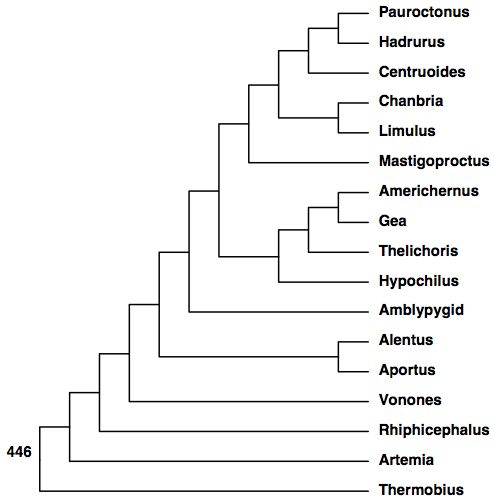
\includegraphics[width=\textwidth]{figures/pstree.jpg}
   	\end{minipage}
\caption{Visualizing trees. An ascii tree (left) is generated using the command \commandstyle{asciitrees}. The same tree is reported to a file in a postscript format (right) using \commandstyle{report("my\_first\_tree", graphtrees)}. Note that both representations of trees  are preceded by their costs.}
\label{fig:trees}
\end{figure}

\section{Creating and running \poy scripts}

So far, we have communicated with \poy interactively through the \emph{Graphical User Interface} or by executing commands from the \emph{Interactive Console}. Another way of conducting an analysis is to run a \emph{script}, a simple-text file containing a list of commands to be performed (Figure~\ref{fig:script}). 

Running analyses using scripts has many advantages: not only does it allow for the entire analysis to proceed from the beginning to the end at one click of a button, it also provides means for examining the logical dependency of the commands (see the description of \poyargument{script\_analysis} argument of the command \poycommand{report} in the \emph{POY Commands} chapter). Submitting jobs using scripts typically produces results faster because \poy automatically optimizes the workflow of the entire analysis by taking into account the functional relationships among various tasks and efficiently distributing the resources (such as memory and multiple processors).

Another advantage of using scripts is that it can contain comments that are ignored by \poy but can be helpful to describe the contents of the files used and provide any other annotations. The comments are enclosed in parenthesis \emph{and} asterisks. For example, \texttt{(*this is a comment*)}. Comments can also be entered interactively from the \emph{Interactive Console}. Their utility in that context is, however, limited unless the comments are featured in some output files.

Obviously, using scripts requires the user to design the workflow of the process prior to conducting the analysis. \poy scripts can be created and saved using \emph{Script Editor} window of \poy interface or any conventional text editor or word processor (such as TextPad, TextWrangler, BBEdit, Emacs, MicrosoftWord, WordPad, or NotePad).

The scripts can be imported and executed using the \emph{POY Launcher} of the \emph{Graphical User Interface}, using the \commandstyle{run()} of the \emph{Interactive Console}or, at start up, by entering the names of the script files (without quotes and parentheses). This is extremely useful in cases when operations may take long time to complete eliminating waiting for a part of the analysis to finish in order to proceed to the next step.

There are three ways to import and run a script:
\begin{itemize}
    \item using the \emph{POY Launcher} of the \emph{Graphical User Interface};
    \item using the \commandstyle{run()} of the \emph{Interactive Console} (such as \texttt{run("script.txt")}, where \texttt{script.txt} is the name of the file containing the script);
   \item from the command line used to start \poy by including the filename(s) of the script (or multiple scripts) (such as \texttt{poy script.txt}.
\end{itemize}

It it critical to include the command \commandstyle{exit()} at the end of the script; otherwise \poy will be waiting for further instructions to be entered after executing the script's contents.

\begin{figure}
\centering
\begin{minipage}[c]{0.42\textwidth}
   		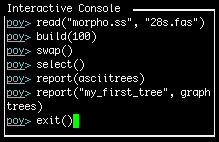
\includegraphics[width=\textwidth]{figures/commandlist.jpg}
\end{minipage}
\quad
\begin{minipage}[c]{0.53\textwidth}
	   	\includegraphics[width=\textwidth]{figures/script.jpg}
   	\end{minipage}
\caption{Using \poy scripts. Executing the list of commands the \emph{Interactive Console} (left)  is equivalent to running a script containing the same list (right). Note, that the header of the script is a comment, inclosed in ``(* *)'', that is ignored by \poy. Also note, that commands can either be listed in a row or in a column (compare \commandstyle{build()} and \commandstyle{swap()} in the console and in the script) and different arguments of the same command can either be specified separately or combined in a single argument list (compare \commandstyle{report()} in the console and in the script). (Both conventions are valid for interactive command submission and for scripts.)}
\label{fig:script}
\end{figure}

\section{Known issues}{\label{sec:known_issues}}

The following issues are known to occur in this beta release. The
core \poy development group is presently working on fixing these
issues.

\begin{enumerate}
    \item If the window is resized during a search, it will not be updated until
        the job is finished.
    \item The diagnosis report is rudimentary but will be greatly expanded in the next version.
    \item The analysis of static homology characters is slow.
    \item The output of the flat interface is reported differently than that of the
        ncurses interface.
    \item The parallel version reports the number of jobs currently running on only 
        \emph{one} of the processors, not in all of them.
\end{enumerate}
